\documentclass[a4paper,12pt]{article} 
\usepackage[ngerman]{babel}
\usepackage{graphicx}
%\usepackage{amsmath}
\begin{document}

{\Large\bf Autonomes Automobil}

\medskip

Quentin Kniep, Timo Redweik, Nicolas Schmitt

\medskip

Friedrich-Wilhelm-Gymnasium K\"oln, Severinstr. 241, 50676 K\"oln

\medskip

5. April  2015

\medskip

{\bf  Abstract}
{\small We solve all problems. No questions remain.}

\medskip

{\bf  Zusammenfassung}
{\small Wir l\"osen alle Probleme. Es bleiben keine Fragen.}

\medskip

{\bf  Keywords:}
{\small Gl\"uck, Geld, Sorgenfreies Leben}

\bigskip


\section{Einf\"uhrung}\label{sec1}

Ziel unseres Projekts war es, ein Modellauto so zu programmieren, dass es selbst\"andig fahren und Hindernissen ausweichen kann.
Dazu haben wir einen Computer in das Auto eingebaut und diesen mit dem Motor verbunden.
Zus\"atzlich haben wir Ultraschallsensoren f\"ur die Abstandsmessung eingebaut.

Ein grundlegender Schaltplan ist in Abb.~\ref{Fig1} vereinfacht dargestellt.

\begin{figure}[h]
	\centering
	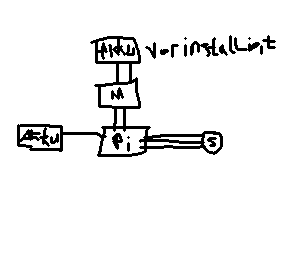
\includegraphics[width=6cm]{./Graphics/Fig1.png}
	\caption{grundlegender Schaltplan}
	\label{Fig1}
\end{figure}

Die wichtigsten Teilaspekte haben wir in Tabelle~\ref{Tab1} zusammengefasst.

\begin{table}[h]
	\centering
	\begin{tabular}{|c|c|c|}
	\hline
		Gl\"uck & Geld  & Sorgenfreies Leben  \\ \hline
		Ja  & Ja & Jaja \\ \hline
	\end{tabular}
	\caption{Sinnfindung}
	\label{Tab1}
\end{table}


\section{Hauptteil}\label{sec2}

Zuerst haben wir das Problem analysiert und das Arbeitsprogramm erstellt.

\subsection{Hauptteil Unterabschnitt}\label{sec2.1}

Der erste Arbeitsunterpunkt wurde so behandelt und folgender L\"osung zugef\"uhrt.

\subsection{Hauptteil Unterabschnitt}\label{sec2.2}

Der zweite Arbeitsschritt f\"uhrte uns auf eine bezaubernde Gleichung

\begin{equation}
	E = mc^2 ,
\end{equation}

die der Kollege Albert vom Patentamt Bern  \cite{Alb05} auch schon beschrieben hat.


\section{Fazit und Ausblick}\label{sec3}

Alles hat wunderbar geklappt. Nichts ging schief und alle sind happy.


\bigskip


{\large\bf Danksagung}

\bigskip


{\large\bf Erkl\"arung der Eigenst\"andigkeit}

\bigskip


\begin{thebibliography}{99}
	\itemsep-2pt \small\frenchspacing
	\bibitem{Alb05}A. Einstein, Annalen der Physik {\bf 18}, 639 (1905).
	\newline
	\bibitem{Alb06}A. Einstein, Annalen der Physik {\bf 18}, 639 (1906).
\end{thebibliography}


\end{document}
